\documentclass[ignorenonframetext,xcolor=x11names]{beamer}

\input{../common.preamble.beamer.tex}
 
\title{Business 4720 - Class 7}

\subtitle{Data Visualization with R}

\begin{document}

\begin{frame}{}
  \titlepage
  \footnotesize 
  \input{../license.tex} 
  
XKCD comics are copyright by their creator (\url{www.xkcd.com}) and licensed under CC-BY-NC
\end{frame}

\begin{frame}{This Class}

\begin{block}{What You Will Learn:}
\begin{itemize}
  \item Introduction to Visualization
  \item Visualizing data with R using the ggplot2 library
\end{itemize}
\end{block}
\end{frame}


\begin{frame}{Why Visualize?}
  \begin{quote} \large \centering
    ''A Picture is Worth 1000 Words''
  \end{quote}
  
\begin{itemize}
  \item Humans are good at visual pattern recognition, but
  \begin{itemize}
    \item Humans also identify patterns where there are none!
    \item It's easy to mislead or deceive with visualization (others and oneself!)
  \end{itemize}
\end{itemize}
\end{frame}

\begin{frame}{Why Visualize?}
\begin{block}{Visual Discovery: Sense Making}
  \begin{itemize}
  \item \alert{Exploration}, confirmation, or verification
  \item Iterative, dynamic
  \end{itemize}
\end{block}

\begin{block}{Declarative Visualization: Storytelling}
  \begin{itemize}
  \item \alert{Explanation}
  \item Affirming, convincing
  \item Presenting, explaining
  \item Decision support
  \item Static
  \end{itemize}
\end{block}

\begin{block}{Operational Visualization: Monitoring}
	\begin{itemize}
		\item Supervision, alarms
		\item Operational decision making
	\end{itemize}
\end{block}
\end{frame}

\begin{frame}{Purpose of Visualization}
\begin{itemize}
  \item Simplify, summarize \& abstract
  \item Compare
  \item Identify trends, patterns \& relationships
  \item Gain insights
\end{itemize}
\end{frame}

\begin{frame}{Quantitative Messages}
\begin{enumerate}
   \item Time-series (e.g. line chart)
   \item Ranking (e.g. bar chart)
   \item Part-whole (e.g. pie chart)
   \item Deviation (e.g. bar chart)
   \item Frequency distribution (e.g. histogram, boxplot)
   \item Correlation (e.g. scatter plot)
   \item Nominal comparison (e.g. bar chart)
   \item Geographic distribution (e.g. cartogram)
\end{enumerate}
\end{frame}

\begin{frame}{Honesty in Visualization}
\begin{block}{General Guidelines}
	\begin{itemize}
		\item Do not deceive your target audience
		\item Do not diminish or hide relationships or trends
		\item Do not exaggerate relationships or trends
		\item Do not confuse or obfuscate
	\end{itemize}
\end{block}
\end{frame}

\begin{frame}{Honesty in Visualization}
\begin{block}{Specific ''no-nos''}
	\begin{itemize}
		\item Graph unrelated data to suggest non-existent relationships
		\item Scale multiple vertical axes to suggest correlations
		\item Truncate or scale axes to hide or exaggerate trend
		\item Scale in multiple dimensions
		\item Plot cumulative growth to hide trend
		\item Use maps for non-geographic data
		\item Use incomplete data (''cherry-picking'')
		\item Use invalid data
	\end{itemize}	
\end{block}
\end{frame}

\begin{frame}{Label your Axes (XKCD)}
  \includegraphics[width=\textwidth]{xkcd_convincing.png}
\end{frame}

\begin{frame}{Use Meaningful Data (XKCD)}
  \includegraphics[width=\textwidth]{xkcd_self_description.png}
\end{frame}

\begin{frame}{Use Related Data (XKCD)}
  \includegraphics[width=\textwidth]{xkcd_coronavirus_charts.png}
\end{frame}

\begin{frame}{Do Not Mislead (XKCD)}
\centering
  \includegraphics[height=3.5in]{xkcd_curve_fitting.png}
\end{frame}

\begin{frame}{Choose Your Axes Meaningfully}
\centering
  \includegraphics[height=3.2in]{xkcd_y_axis_2x.png}
\end{frame}

\begin{frame}{Be Careful When Extrapolating (XKCD)}
\centering
  \includegraphics[width=\textwidth]{xkcd_extrapolating.png}
\end{frame}

\begin{frame}{Verify Trends (XKCD)}
\centering
  \includegraphics[width=\textwidth]{xkcd_linear_regression.png}
\end{frame}

\begin{frame}{Use Appropriate Scales (XKCD)}
\centering

  \includegraphics[width=\textwidth]{xkcd_log_scale.png}
\end{frame}

\begin{frame}{Don't Lose Your Point}
\centering
  \includegraphics[height=3.3in]{xkcd_tall_infographics.png}
\end{frame}

\begin{frame}{Dark Patterns -- Truncated Axes}
\centering
\includegraphics[width=\textwidth]{screen3.png}

\scriptsize\url{https://en.wikipedia.org/wiki/Misleading_graph}
\end{frame}

\begin{frame}{Dark Patterns -- Omitted Data}
\centering
\includegraphics[width=\textwidth]{screen5.png}

\scriptsize\url{https://en.wikipedia.org/wiki/Misleading_graph}
\end{frame}

\begin{frame}{Dark Patterns -- 3D Pie Charts}
\centering
\includegraphics[width=\textwidth]{screen6.png}

\scriptsize\url{https://en.wikipedia.org/wiki/Misleading_graph}
\end{frame}

\begin{frame}{Dark Patterns -- Comparing Pie Charts}
\centering
\includegraphics[width=\textwidth]{screen7.png}

\scriptsize\url{https://en.wikipedia.org/wiki/Misleading_graph}
\end{frame}

\begin{frame}{Dark Patterns -- Scaling Axes and Aspect Ratios}
\centering
\includegraphics[width=\textwidth]{screen4.png}

\scriptsize\url{https://en.wikipedia.org/wiki/Misleading_graph}
\end{frame}

\begin{frame}{Dark Patterns -- Scaling Multiple Dimensions}
\centering
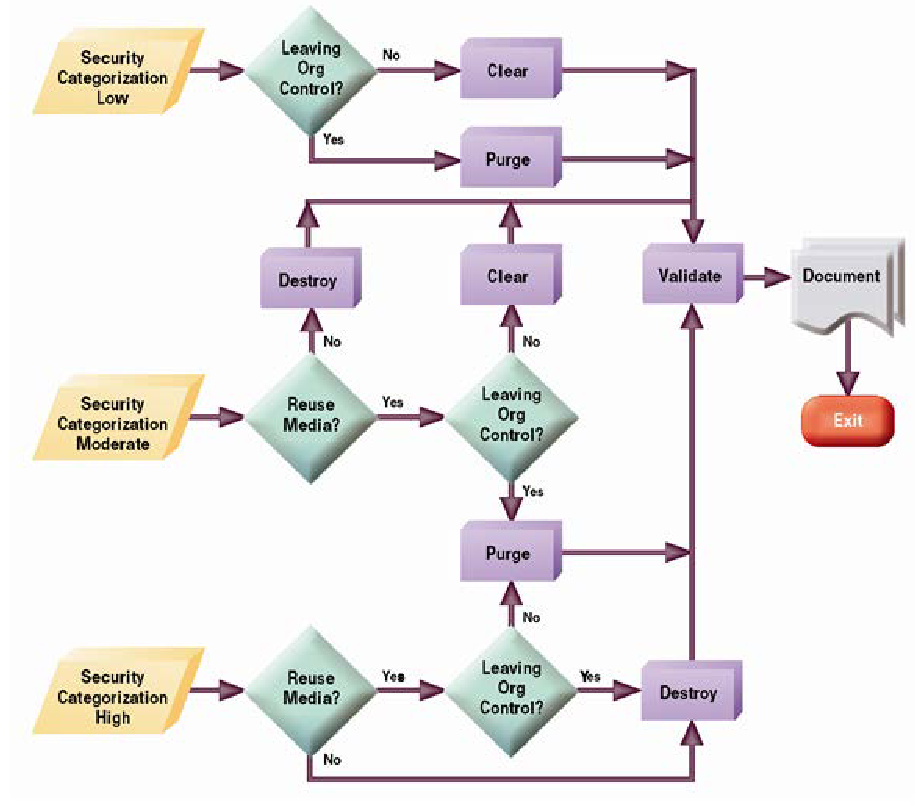
\includegraphics[width=\textwidth]{screen1.png}

\scriptsize\url{https://en.wikipedia.org/wiki/Misleading_graph}
\end{frame}

%\begin{frame}{Special Types of Data and Visual Analytics}
	%\begin{itemize}
		%\item Streaming data
		%\begin{itemize}
			%\item Continually changing
			%\item Limited buffers/windows
		%\end{itemize}
		%\item Spatial, geographic, map data
		%\begin{itemize}
		   %\item Geo aware, irregular map boundaries, image overlays
		%\end{itemize}
		%\item Network data
		%\begin{itemize}
		   %\item Vertices and vertex types, edges and edge types
		%\end{itemize}
		%\item Text data
		%\begin{itemize}
		   %\item Unstructured text, e.g. from social media or web sites
		%\end{itemize}
	%\end{itemize}
%\end{frame}

\begin{frame}{Colour Palettes}
\begin{itemize}
   \item Colour is an important visualization element
   \item A colour palette defines a set of colours for a graph/plot.
\end{itemize}
\begin{block}{Desirable Characteristics}
\begin{itemize} 
  \item Colourful (range of values)
  \item Perceptually uniform (even perceptual distances)
  \item Robust to colourblindness (CVD)
  \item Pretty
\end{itemize}
\end{block}
\end{frame}

\begin{frame}{Types of Colour Palettes}
\begin{block}{Sequential/Monochrome}
\begin{itemize}
  \item Varying hue, light to dark/deep
  \item Discrete or continuous
  \item Show progression for data with inherent order
\end{itemize}
\begin{center}
  \includegraphics[width=.7\textwidth]{monochromatic.pdf}
  \includegraphics[width=.7\textwidth]{sequential.pdf}
\end{center}
\end{block}
\end{frame}

\begin{frame}{Types of Colour Palettes \small [cont'd]}
\begin{block}{Divergent}
\begin{itemize}
  \item From one colour to another via white or black
  \item Discrete or continuous
  \item Useful for showing deviations or extremes on either size of midpoint
  \item Data with meaningful center
\end{itemize}
\begin{center}
  \includegraphics[width=.7\textwidth]{diverging.pdf}
\end{center}
\end{block}
\end{frame}

\begin{frame}{Types of Colour Palettes \small [cont'd]}
\begin{block}{Spectral}
\begin{itemize}
  \item Uses a number of different colours
  \item Discrete
  \item Data without inherent ordering
  \item Limited to few categories as colours become too similar
\end{itemize}
\begin{center}
  \includegraphics[width=.7\textwidth]{brewer.paired.pdf}
\end{center}
\end{block}
\end{frame}

\begin{frame}{CVD (Colour Vision Deficiency)}
\begin{itemize}
  \item Monochromatism
  \item Protanopia (missing ''S-cone'', blue)
  \item Deuteranopia (missing ''M-cone'', green)
  \item Tritanopia (missing ''L-cone'', red)
\end{itemize}
\vspace{1cm}
\centering
1 in 12 men have CVD \\
1 in 200 women have CVD \\
2.6 million Canadians are colour blind
\end{frame}

\begin{frame}{Original}
  \includegraphics[width=\textwidth]{photo.jpg}
  \centering
  MUN Faculty of Education Class Room \\
  {\tiny Copyright Memorial University of Newfoundland}
\end{frame}

\begin{frame}{Simulated Colour Vision Deficiencies}
\begin{tabular}{cc} 
  \includegraphics[width=.48\textwidth]{desaturate\_photo.jpg} &
  \includegraphics[width=.48\textwidth]{protan\_photo.jpg} \\ 
  Monochromatism & Protanopia \\ 
  \includegraphics[width=.48\textwidth]{deutan\_photo.jpg} &
  \includegraphics[width=.48\textwidth]{tritan\_photo.jpg} \\ 
  Deuteranopia & Tritanopia \\ 
\end{tabular}
\end{frame}
    
\begin{frame}{Example: Colourbrewer Palette ''Paired''}
  \includegraphics[width=\textwidth]{brewer.paired.cvd.pdf}
\end{frame}

\begin{frame}{Viridis Colour Palette}
  \includegraphics[width=\textwidth]{viridis.plot.pdf}
\end{frame}


%\begin{frame}{Plots for One Variable}
%\begin{block}{Continuous}
%\begin{itemize}
  %\item {\bf Area}: Degree of change over time, or relationship of parts to aggregate
  %\item {\bf Density, Dot, Frequency, Histogram}: Show frequency distribution of data
%\end{itemize}
%\end{block}

%\begin{block}{Discrete}
%\begin{itemize}
  %\item {\bf Bar}: Connections among individual things, compare items of different groups
  %\item {\bf Pie}: Relationships of parts to aggregate
%\end{itemize}
%\end{block}
%\end{frame}

%\begin{frame}{Plots for Two Variables}
%\begin{block}{Both Continuous}
%\begin{itemize}
  %\item {\bf Point}: Connections among numeric values, show multiple groups of data
  %\item {\bf Lines, Local Regression}: Relationships/correlations among multiple data series or over time
  %\item {\bf Text / Label}: Frequency of labels in content/document
%\end{itemize}
%\end{block}

%\begin{block}{One Discrete, One Continuous}
%\begin{itemize}
  %\item {\bf Column}: Correlations among things or information changes over time
  %\item {\bf Box, Dot, Violin}: Compare distributions between many groups, display spread and skew of data
%\end{itemize}
%\end{block}
%\end{frame}

%\begin{frame}{Plots for Two Variables, cont'd}
	%\begin{block}{Both Discrete}
		%\begin{itemize}
			%\item {\bf Points/Counts}: Magnitude of counts
			%\item {\bf Jitter}: Plots of data points
		%\end{itemize}
	%\end{block}
	%\begin{block}{Distributions}
		%\begin{itemize}
			%\item {\bf Bin2D, Density2D, Hex}: Shows frequency of values over two continuous variables
		%\end{itemize}
	%\end{block}
%\end{frame}

%\begin{frame}{Plots for Three Variables}
	%\begin{block}{Continuous}
		%\begin{itemize}
			%\item {\bf Contour, Raster and Tile}: Shows relationships among three data series
		%\end{itemize}
	%\end{block}
%\end{frame}

%\begin{frame}{Visualizing Errors and Uncertainty}
%\begin{block}{Purpose}
	%\begin{itemize}
		%\item Give a general idea of how precise a value is, or how far a value might be from the true value
		%\item Used to augment a given visualization
	%\end{itemize}
%\end{block}
%\begin{block}{Common Visualization Styles}
%\begin{itemize}
  %\item Crossbar
  %\item Errorbar
  %\item Range (line, point)
%\end{itemize}  
%\end{block}
%\end{frame}

\begin{frame}{Popular Graphics Libraries and Frameworks}
\begin{block}{R}
\begin{itemize}
  \item GGPlot (and related libraries such as GGPattern)
  \item Plotly for R
  \item GGVis (for Dashboards)
  \item Shiny (for Dashboards)
\end{itemize}
\end{block}
\begin{block}{Python}
\begin{itemize}
  \item Matplotlib
  \item Seaborn
  \item Plotly (Express, GO, Dash)
  \item Plotnine (''GGPlot for python'')
  \item Shiny (for Dashboards)
\end{itemize}
\end{block}
\begin{block}{Web \& JS}
\begin{itemize}
  \item D3, ChartJS, GoogleCharts
\end{itemize}
\end{block}
\end{frame}

\begin{frame}{Plot Elements}
	\begin{block}{Map Data to Plot Elements}
	\begin{itemize}
		\item X, Y axis
		\item Colour (point, line, fill)
		\item Transparency (''alpha'')
		\begin{itemize}
		   \item \alert{Be aware of print versus screen or color vision deficiency}
		\end{itemize}
		\item Pattern (fill)
		\item Size, Weight/Width (point, line)
		\item Shape, Style (point, line)
	\end{itemize}
	\end{block}
	\begin{block}{Other Plot Elements}
		\begin{itemize}
			\item Title, sub-title, captions
			\item Axis titles, axis labels and ''ticks''
			\item Legend(s)
		\end{itemize}
	\end{block}
\end{frame}

\begin{frame}{Example Dataset}
\begin{itemize}
  \item Government of Canada, Open Government Portal
  \item Fuel Consumption Ratings -- Battery-electric vehicles -- 2012--2023; last updated Oct 10, 2023
  \item \href{https://open.canada.ca/data/en/dataset/98f1a129-f628-4ce4-b24d-6f16bf24dd64}{https://open.canada.ca/data/en/dataset/98f1a129-f628-4ce4-b24d-6f16bf24dd64}
\end{itemize}
\centering
\footnotesize

	\begin{tabular}{|l|l|} \hline
	  {\bf Column} & {\bf Data Type} \\ \hline \hline
	  Make & Discrete \\ 
	  Model & Discrete \\
	  Year & Numeric \\
	  Category & Discrete \\
	  City & Numeric\footnote{Fuel consumption in l/100km equivalent} \\
	  Hwy & Numeric \\
	  Comb & Numeric \\
	  Range & Numeric\footnote{Range in km} \\ \hline
	\end{tabular}
\end{frame}

\begin{frame}[fragile]{Example Dataset -- Read Data}
\begin{Rcode}
# Load tidyverse package
library(tidyverse)

# Read the data set to a Tibble
data <- read_csv('https://evermann.ca/busi4720/fuel.csv')

# Ensure vehicle category is a factor (categorical)
data$Fuel <- as.factor(data$Fuel)
\end{Rcode}
\end{frame}

\begin{frame}[fragile]{Load Graphics Libraries}
\small
\begin{Rcode}
library(ggplot2)
library(ggpattern)
library(ggstream)
library(ggsci)
library(scales)
library(ggrepel)
library(ggradar)
\end{Rcode}
\end{frame}

\begin{frame}[fragile]{Histogram}

\begin{Rcode}
data |> 
  ggplot(aes(x=Range)) + 
    geom_histogram(bins=50)
\end{Rcode}

\begin{itemize}
  \item Aesthetic \texttt{aes()} determines mapping of data to plot elements
  \item Add ''geoms'' that determine the type of plot
  \item Geoms can have their own additional aesthetics and other options
\end{itemize}

\begin{Rcode}
ggsave("histogram.pdf", height=5, width=7.5, units='in')
\end{Rcode}

\begin{itemize}
  \item Save plot in different formats (PDF, PNG, JPEG, \ldots)
\end{itemize}
\end{frame}

\begin{frame}{Histogram}
\begin{columns}
\begin{column}{.75\textwidth}
  \includegraphics[width=\textwidth]{histogram.pdf}
\end{column}
\begin{column}{.35\textwidth}
\footnotesize
\begin{itemize}
\item Shows frequencies or counts
\end{itemize}
\end{column}
\end{columns}
\end{frame}

\begin{frame}[fragile]{Density Plot}

\begin{Rcode}
data |> 
  ggplot(aes(Range)) + 
    geom_density(kernel='gaussian', fill='lightblue')
\end{Rcode}
\begin{columns}
\begin{column}{.75\textwidth}
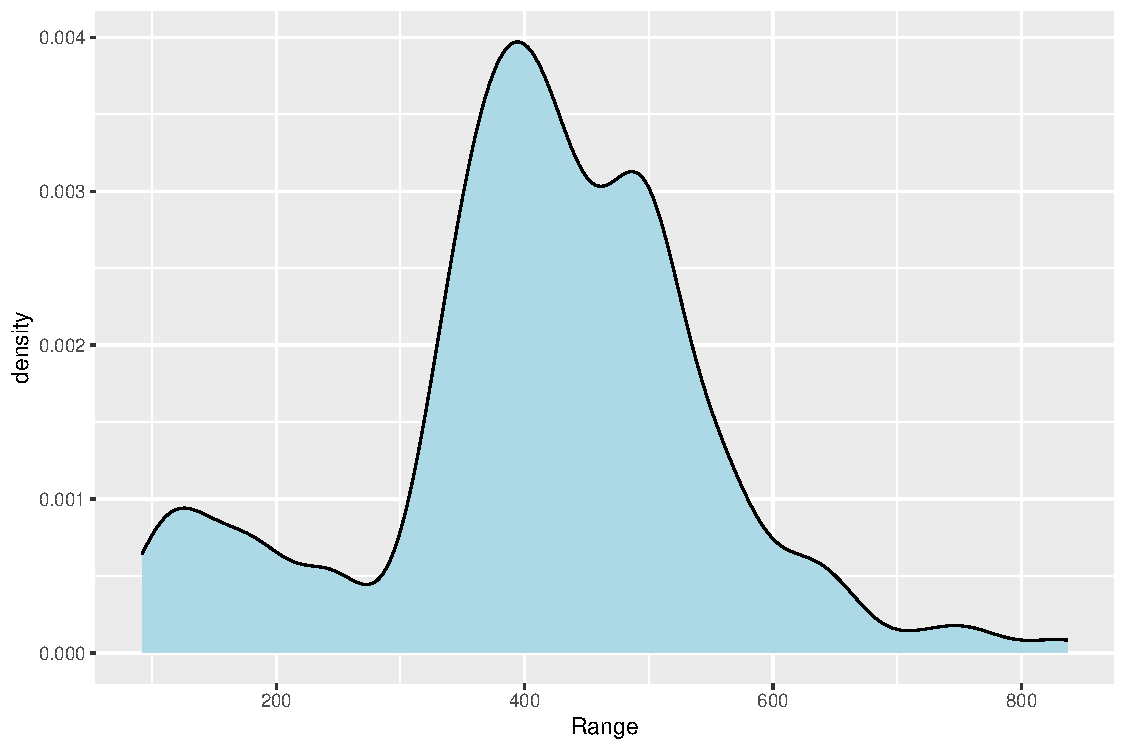
\includegraphics[width=\textwidth]{fuel.density.simple.pdf}
\end{column}
\begin{column}{.35\textwidth}
\footnotesize
\begin{itemize}
\item Shows probability density functions
\item Kernel is used to smooth the curve (how to weight points)
\end{itemize}
\end{column}
\end{columns}
\end{frame}

\begin{frame}[fragile]{Combining Geoms}
\begin{Rcode}
data |> ggplot(aes(Range)) +
    geom_density(kernel='gaussian', 
        alpha=0.25, fill='lightblue') +
    geom_histogram(aes(y=after_stat(density)), bins=50, 
        alpha=0.5, fill='white', color='black')
\end{Rcode}
\begin{columns}
\begin{column}{.75\textwidth}
  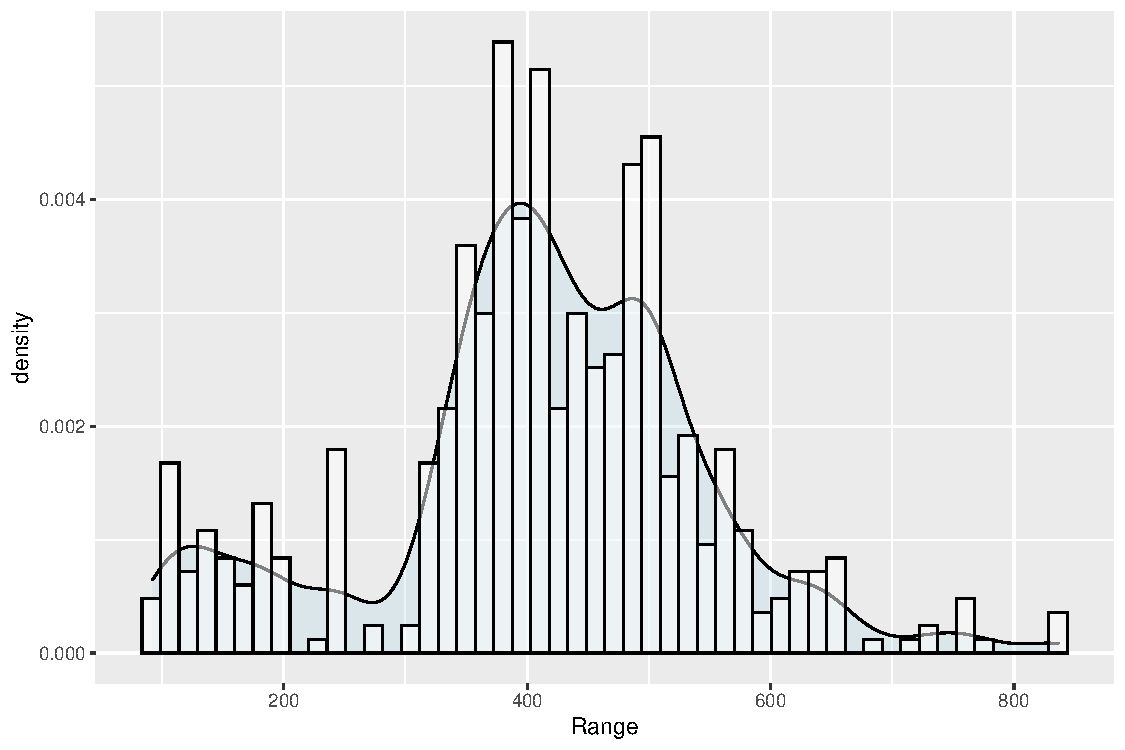
\includegraphics[width=\textwidth]{fuel.histogram.pdf}
\end{column}
\begin{column}{.35\textwidth}
\footnotesize
\begin{itemize}
    \item The \texttt{alpha} option controls transparency
\end{itemize}
\end{column}
\end{columns}
\end{frame}

\begin{frame}[fragile]{Labelling}
\begin{Rcode}
data |>  ggplot(aes(x=Range)) + 
    geom_histogram(bins=50) +
    labs(x = 'Range in km',
         y = 'Number of vehicle models',
         title='Number of Vehicle Models by Vehicle Range',
         subtitle='Years 2012 to 2024',
         caption='From NRCAN Data')
\end{Rcode}
\begin{center}
  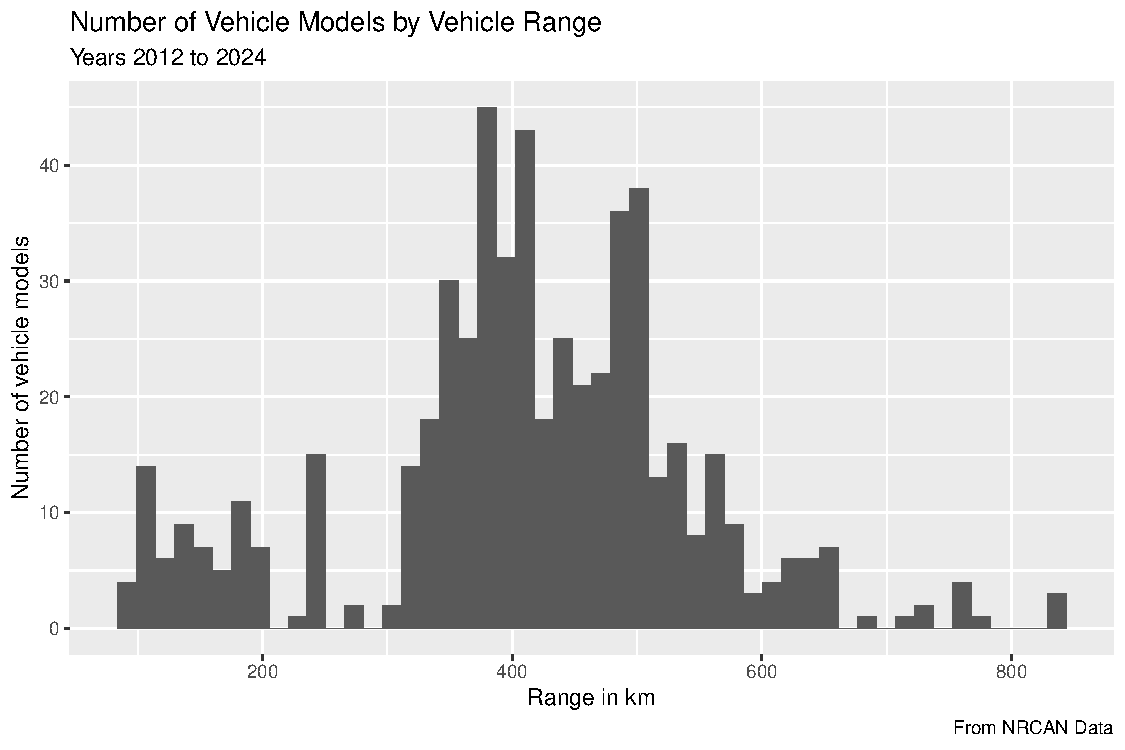
\includegraphics[width=.7\textwidth]{fuel.histogram.labels.pdf}
\end{center}
\end{frame}

%\begin{frame}[fragile]{Complex Example -- Multiple Geoms}
%Prepare some summary statistics:

%\small
%\begin{Rcode}
%# Calculate summary statistics for Range variable
%mean_v <- data |>
   %summarize(mean_v = mean(Range), 
             %median_v = median(Range), 
             %lower95=quantile(Range, .025), 
             %upper95=quantile(Range, .975), 
             %maxdensity = max(density(Range)$y))
%\end{Rcode}
%\end{frame}

%\begin{frame}[fragile]{Complex Example -- Multiple Geoms \small [cont'd]}
%\footnotesize
%\begin{Rcode}
%data |> 
  %ggplot(aes(Range)) + 
    %geom_density(fill='lightblue') + 
    %labs(x = 'Range (km)', 
         %y = 'Proportion of Vehicles', 
         %title='Density Plot - Electric Vehicle Range', 
         %subtitle='Years 2012 to 2024', 
         %caption='95 percentile, median and mean') +
    %geom_vline(data=mean_v, aes(xintercept=mean_v), 
               %linetype='dashed') +
    %geom_vline(data=mean_v, aes(xintercept=median_v), 
               %linetype='dotdash') +
    %geom_vline(data=mean_v, aes(xintercept=lower95), 
               %linetype='dotted') +
    %geom_vline(data=mean_v, aes(xintercept=upper95), 
           %linetype='dotted') + 
%\end{Rcode}
%\end{frame}

%\begin{frame}[fragile]{Complex Example -- Multiple Geoms \small [cont'd]}
%\footnotesize
%\begin{Rcode}
%annotate('text', 
   %label=paste(' L95=\n ',round(mean_v$lower95)), 
   %x = mean_v$lower95, y = mean_v$maxdensity/2, 
   %size=3.5, hjust=0) +
%annotate('text', 
   %label=paste(' Med=\n ',round(mean_v$median_v)), 
   %x = mean_v$median_v, y = mean_v$maxdensity*3/4, 
   %size=3.5, hjust=0) +
%annotate('text',
   %label=paste(' Mean=\n ',round(mean_v$mean_v)), 
   %x = mean_v$mean_v, y = mean_v$maxdensity*5/8, 
   %size=3.5, hjust=0) + 
%annotate('text',
   %label=paste(' U95=\n ',round(mean_v$upper95)), 
   %x = mean_v$upper95, y = mean_v$maxdensity/2, 
   %size=3.5, hjust=0)
%\end{Rcode}
%\end{frame}

%\begin{frame}{Complex Example -- Multiple Geoms  [cont'd]}
%\begin{columns}
%\begin{column}{.75\textwidth}
  %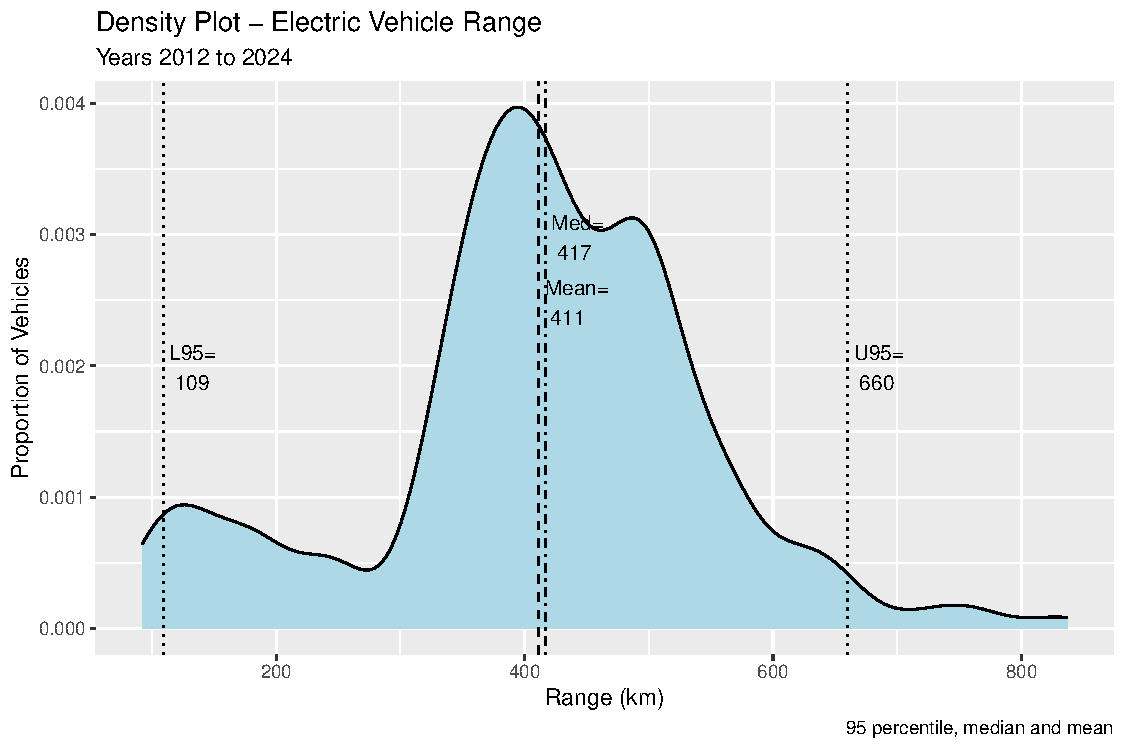
\includegraphics[width=\textwidth]{fuel.density.pdf}
%\end{column}
%\begin{column}{.35\textwidth}
%\footnotesize
%\begin{itemize}
   %\item \texttt{geom\_vline} and \texttt{annotate} are geoms
   %\item \texttt{geom\_vline} specifies \texttt{data=mean\_v} data frame
%\end{itemize}
%\end{column}
%\end{columns}
%\end{frame}

\begin{frame}{Hands-On Exercises}
\begin{block}{}
\begin{enumerate}
    \item Read the EV fuel efficiency data set into R .
    \item Create a blue histogram of highway efficiency with 25 bins.
    \item Add labels for the axes, and add a title.
\end{enumerate}
\end{block}

\begin{block}{Tips}
    \begin{itemize} 
       \item Use the \texttt{read\_csv()} function from the tidyverse library
       \item The column name is \texttt{Hwy}
       \item Use the \texttt{geom\_histogram} geom
       \item Use the \texttt{bins=\ldots} option
       \item Use the \texttt{fill='\ldots'} option
       \item Use the \texttt{labs} geom for labels
    \end{itemize}
\end{block}
\end{frame}


\begin{frame}[fragile]{Area Plot}
\footnotesize
\begin{Rcode}
data %>% group_by(Year) %>%
  summarize(meanRange = mean(Range)) %>% ungroup() %>%
  ggplot(aes(Year, meanRange)) + 
    geom_area(fill='lightgreen') +
    geom_text(aes(label=round(meanRange)), size=5)
\end{Rcode}
\begin{columns}
\begin{column}{.75\textwidth}
  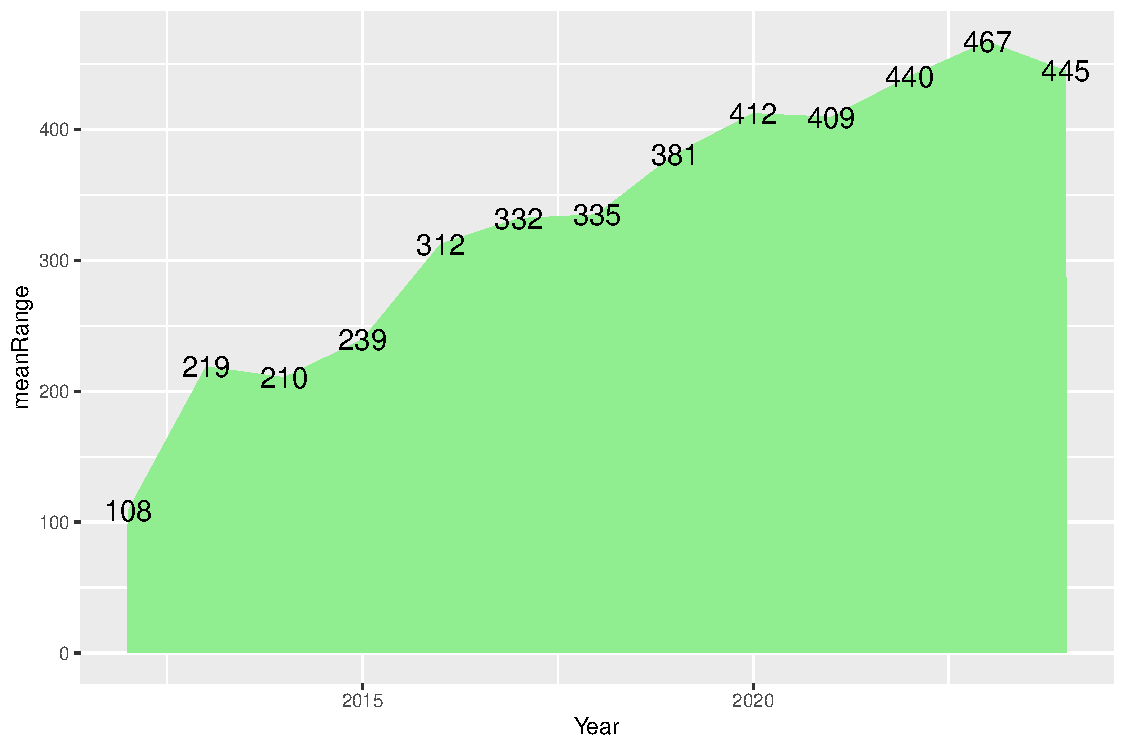
\includegraphics[width=\textwidth]{fuel.areaOneSeries.pdf}
\end{column}
\begin{column}{.35\textwidth}
\begin{itemize}
   \item The \texttt{ggplot()} function is the last in a data processing pipeline
\end{itemize}
\end{column}
\end{columns}
\end{frame}

\begin{frame}[fragile]{Column Chart}
\begin{itemize}
   \item Data must have one variable mapped to Y axis
   \item Data must have one variable mapped to fill colour
\end{itemize}

\begin{columns}
\begin{column}{.6\textwidth}
\begin{Rcode}
col.data <- data %>%
   group_by(Year) %>%
   summarize(
     meanCity = mean(City), 
     meanHwy = mean(Hwy)) %>%
   ungroup() %>%
   pivot_longer(
     cols=c('meanCity', 'meanHwy'), 
     names_to='metric', 
     values_to='consumption')
\end{Rcode}
\end{column}
\begin{column}{.5\textwidth}
\begin{textcode}
   Year meanCity meanHwy
  <dbl>    <dbl>   <dbl>
1  2012     2.05    2.5 
2  2013     2.27    2.5 
3  2014     2.16    2.43
\end{textcode}
\begin{textcode}
   Year metric   consumption
  <dbl> <chr>          <dbl>
1  2012 meanCity        2.05
2  2012 meanHwy         2.5 
3  2013 meanCity        2.27
4  2013 meanHwy         2.5 
5  2014 meanCity        2.16
6  2014 meanHwy         2.43
\end{textcode}
\end{column}
\end{columns}
\end{frame}

\begin{frame}[fragile]{Column Chart \small [cont'd]}
\begin{Rcode}
col.data |> 
   ggplot(aes(x=Year, y=consumption, fill=metric)) +
      geom_col(position='dodge')
\end{Rcode}
\begin{columns}
\begin{column}{.75\textwidth}
  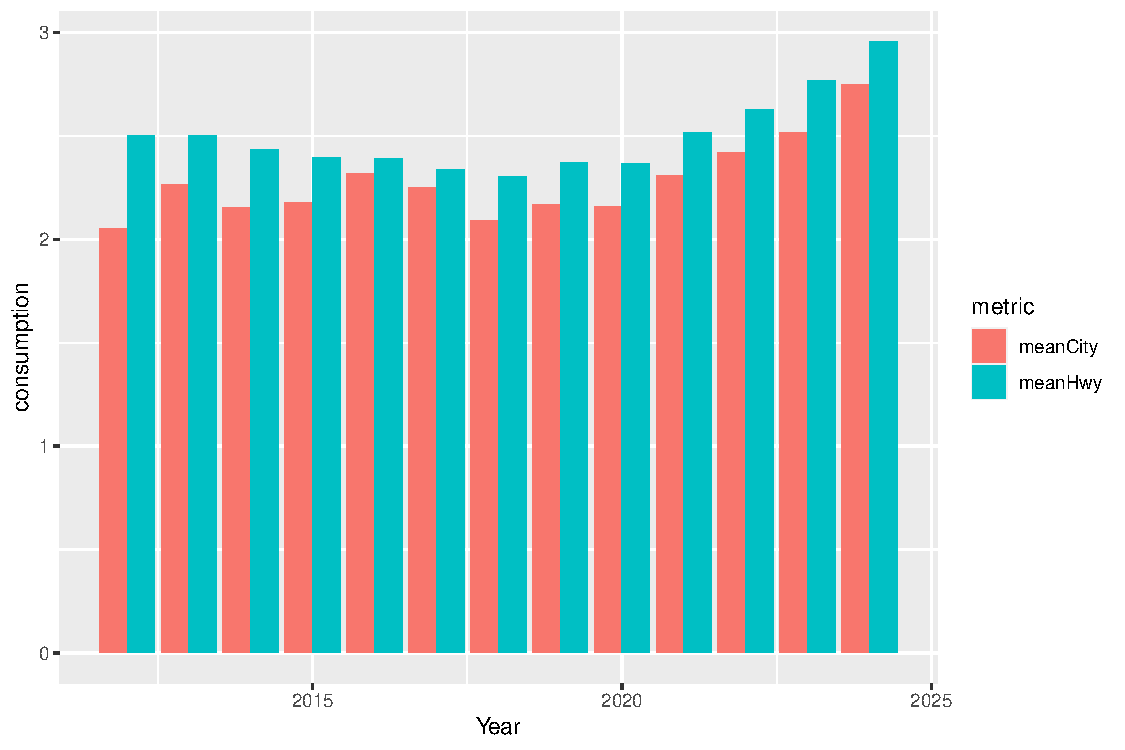
\includegraphics[width=\textwidth]{fuel.columns.pdf}
\end{column}
\begin{column}{.35\textwidth}
\footnotesize
\begin{itemize}
   \item The option \texttt{position = 'dodge'} places the columns next to each other, instead of on top of each other.
\end{itemize}
\end{column}
\end{columns}
\end{frame}


\begin{frame}[fragile]{Column Chart with Patterns}
\begin{Rcode}
col.data |> ggplot(aes(x=Year, y=consumption)) +
    geom_col_pattern(aes(pattern_type=metric),
          pattern='polygon_tiling', pattern_angle=45,
          pattern_fill='white', position='dodge') +
    scale_pattern_type_manual(
       values = c('hexagonal', 'rhombille'), 
       labels=c("City", "Highway"))
\end{Rcode}
\begin{center}
  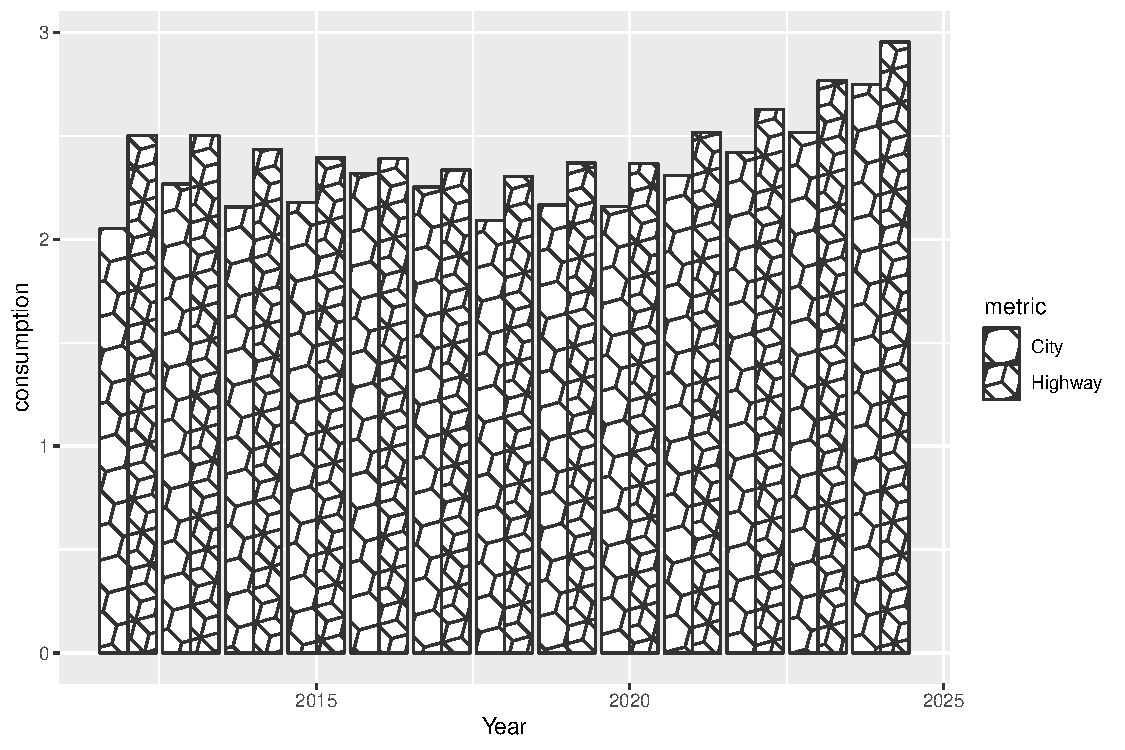
\includegraphics[height=2in]{fuel.columnsPatterns.pdf}
\end{center}
\end{frame}

\begin{frame}[fragile]{Box Plot}

\begin{Rcode}
data |>
  pivot_longer(cols=c('City', 'Hwy'), 
               names_to='metric', values_to='consumption') |>
ggplot(aes(x=as.factor(Year), y=consumption, fill=metric)) +
  geom_boxplot()
\end{Rcode}
\begin{columns}
\begin{column}{.75\textwidth}
  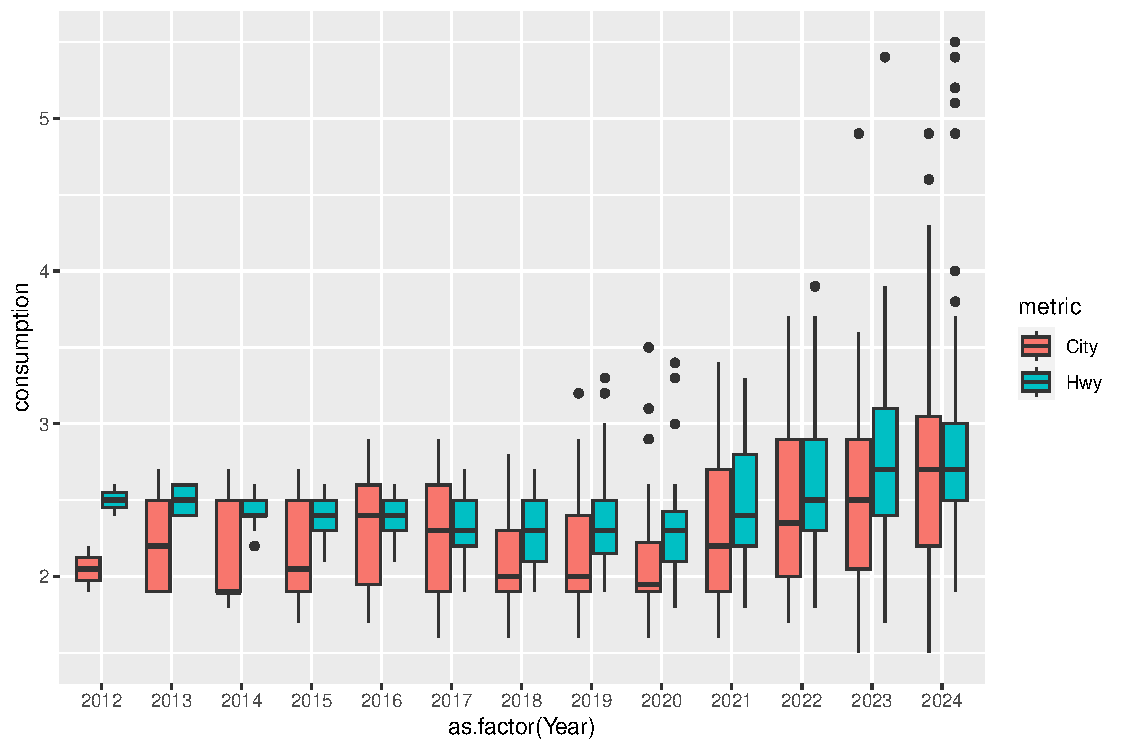
\includegraphics[height=2in]{fuel.box.pdf}
\end{column}
\hspace{-.5in}
\begin{column}{.35\textwidth}
\footnotesize
\begin{itemize}
   \item Shows distribution
   \item Median
   \item 1st quartile $Q_1$
   \item 3rd quartile $Q_3$
   \item ''Inter-quartile range''
   \item $IQR = Q_3 - Q_1$
   \item ''Whiskers''
   \item $Q_3 + 1.5 \times IQR$
   \item $Q_1 - 1.5 \times IQR$
   \item ''Outliers''
\end{itemize}
\end{column}
\end{columns}
\end{frame}


\begin{frame}{Boxplot (XKCD)}
 \includegraphics[width=\textwidth]{xkcd_box_plot.png}
\end{frame}

\begin{frame}[fragile]{Violin Plot}
\begin{Rcode}
data |>
  pivot_longer(cols=c('City', 'Hwy'), 
               names_to='metric', 
               values_to='consumption') |>
  ggplot(aes(x=as.factor(Year), y=consumption, fill=metric)) +
    geom_violin()
\end{Rcode}
\begin{columns}
\begin{column}{.75\textwidth}
  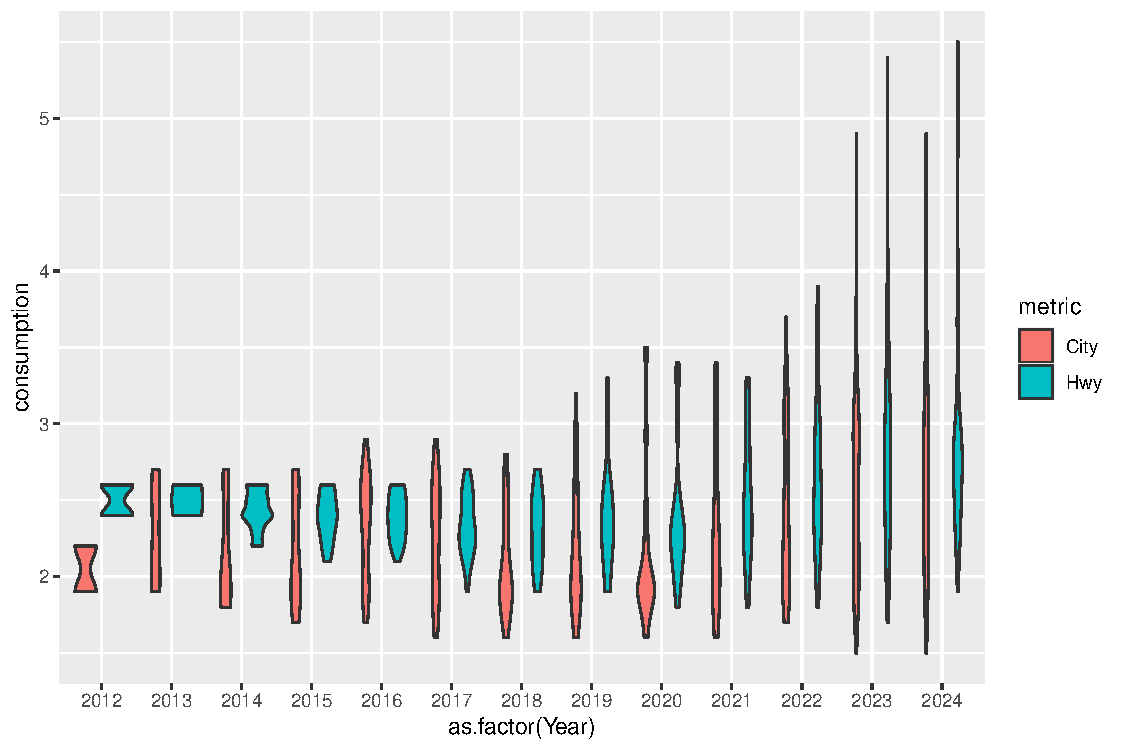
\includegraphics[height=2in]{fuel.violin.pdf}
\end{column}
\hspace{-.75in}
\begin{column}{.25\textwidth}
\footnotesize
\begin{itemize}
   \item Shows detailed density
   \item But no summary statistics
\end{itemize}
\end{column}
\end{columns}
\end{frame}

%\begin{frame}[fragile]{Dot Plot}
%\footnotesize
%\begin{Rcode}
%data %>% 
  %ggplot(aes(x=as.factor(Year), y=Comb)) +
    %geom_dotplot(binaxis='y', 
                 %stackdir='center', 
                 %stackratio=0.5,
                 %binpositions='all',
                 %dotsize=0.5, 
                 %color='black', 
                 %fill='orange') +
    %scale_fill_brewer(palette="Paired") +
    %labs(x = 'Year', 
         %y='Mean Fuel Consumption\n(l/100km equiv)', 
         %fill='', 
         %title='Electric Vehicle Range', 
         %subtitle='Years 2012 to 2024')
%\end{Rcode}
%\end{frame}

%\begin{frame}{Dot Plot}
  %\includegraphics[width=\textwidth]{fuel.dotplot.pdf}
%\end{frame}

%\begin{frame}[fragile]{Dot Plot (with Violin and Range Summary)}
%\footnotesize
%\begin{Rcode}
%data %>% 
  %filter(Year > 2019) %>%
  %ggplot(aes(x=as.factor(Year), y=Comb)) +
    %geom_dotplot(binaxis='y', 
                 %stackdir='center', stackratio=0.5,
                 %binpositions='all', dotsize=0.5, 
                 %color='black', fill='orange') +
    %geom_violin(color='black', fill=NA) + 
    %stat_summary(fun.data=mean_sdl, 
                 %fun.args=list(mult=1), 
                 %size=1, color='blue', 
                 %geom="pointrange") +
    %scale_fill_brewer(palette="Paired") +
    %labs(x = 'Year', 
         %y='Mean Fuel Consumption\n(l/100km equiv)', 
         %fill='', 
         %title='Electric Vehicle Range', 
         %subtitle='Years 2020 to 2024') +
     %theme(legend.position='none')
%\end{Rcode}
%\end{frame}

%\begin{frame}{Dot Plot (with Violin and Range Summary)}
  %\includegraphics[width=\textwidth]{fuel.dotplotjviolinsummary.pdf}
%\end{frame}

\begin{frame}[fragile]{Count Plot}
\begin{Rcode}
data %>% 
ggplot(aes(as.factor(Year), as.factor(Category))) +
    geom_count(color='darkolivegreen4') +
    scale_y_discrete(
      labels=c('Compact', 'Large', 'Mid-Size', 'Pickup truck', 
               'Subcompact', 'Two-seater', 'SUV (standard)', 
               'SUV (small)', 'Station Wagon (small)'))
\end{Rcode}
\begin{columns}
\begin{column}{.65\textwidth}
  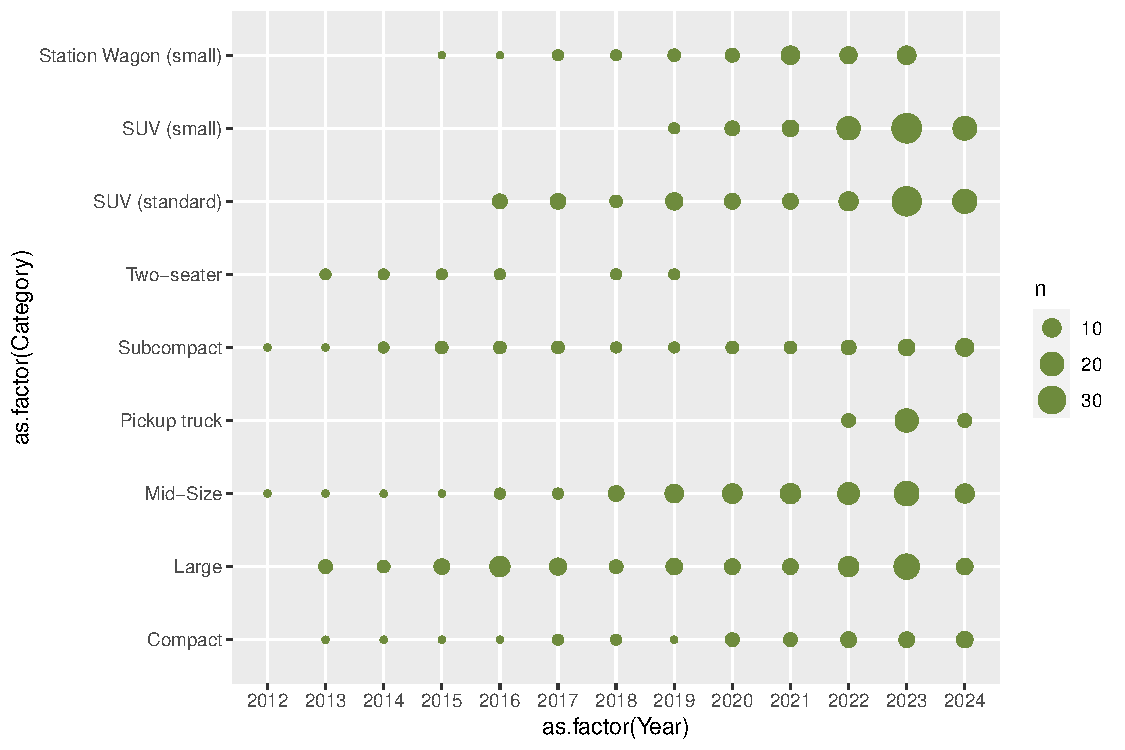
\includegraphics[height=1.75in]{fuel.count.pdf}
\end{column}
\begin{column}{.35\textwidth}
\footnotesize
\begin{itemize}
   \item Explicit labels for discrete y axis
\end{itemize}
\end{column}
\end{columns}
\end{frame}

\begin{frame}[fragile]{Jitter Plot}
\begin{Rcode}
data |> 
  filter(Year >= 2020) |>
  ggplot(aes(x=as.factor(Year), y=as.factor(Category), 
             color=as.factor(Year))) +
    geom_jitter(width=0.2, height=0.2) +
    guides(color='none')
\end{Rcode}
\begin{columns}
\begin{column}{.70\textwidth}
  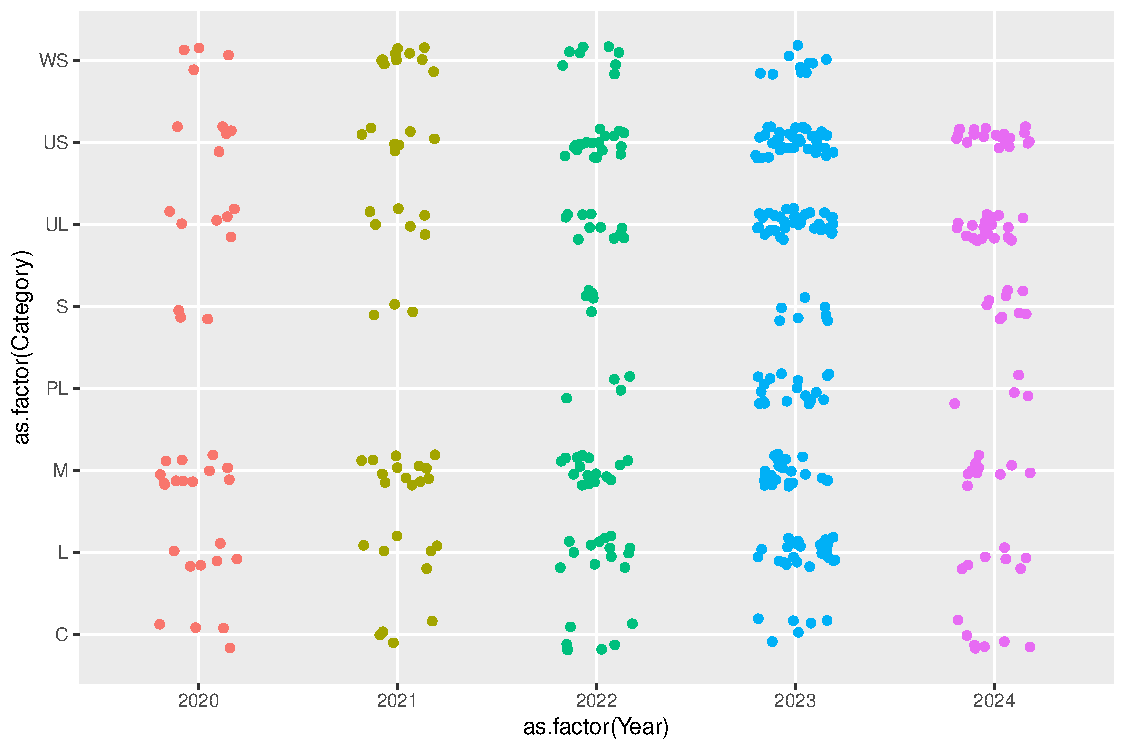
\includegraphics[height=1.75in]{fuel.jitterdiscrete.pdf}
\end{column}
\begin{column}{.35\textwidth}
\footnotesize
\begin{itemize}
   \item Shows all data points (observations)
   \item No legend (''guide'') for different colours
   \item Because colour is also mapped to Year, same as x axis
\end{itemize}
\end{column}
\end{columns}
\end{frame}

\begin{frame}[fragile]{Points Plot}
\begin{Rcode}
data |> 
  group_by(Year, Category) |>
  summarize(totalcount=n(), meanRange=mean(Range)) |>
  ungroup () |>
ggplot(aes(x=as.factor(Year), y=meanRange, 
           size=totalcount, color=Category)) +
  geom_point(alpha=0.8) +
  scale_size_continuous(range=c(0, 20))
\end{Rcode}
\begin{columns}
\begin{column}{.55\textwidth}
  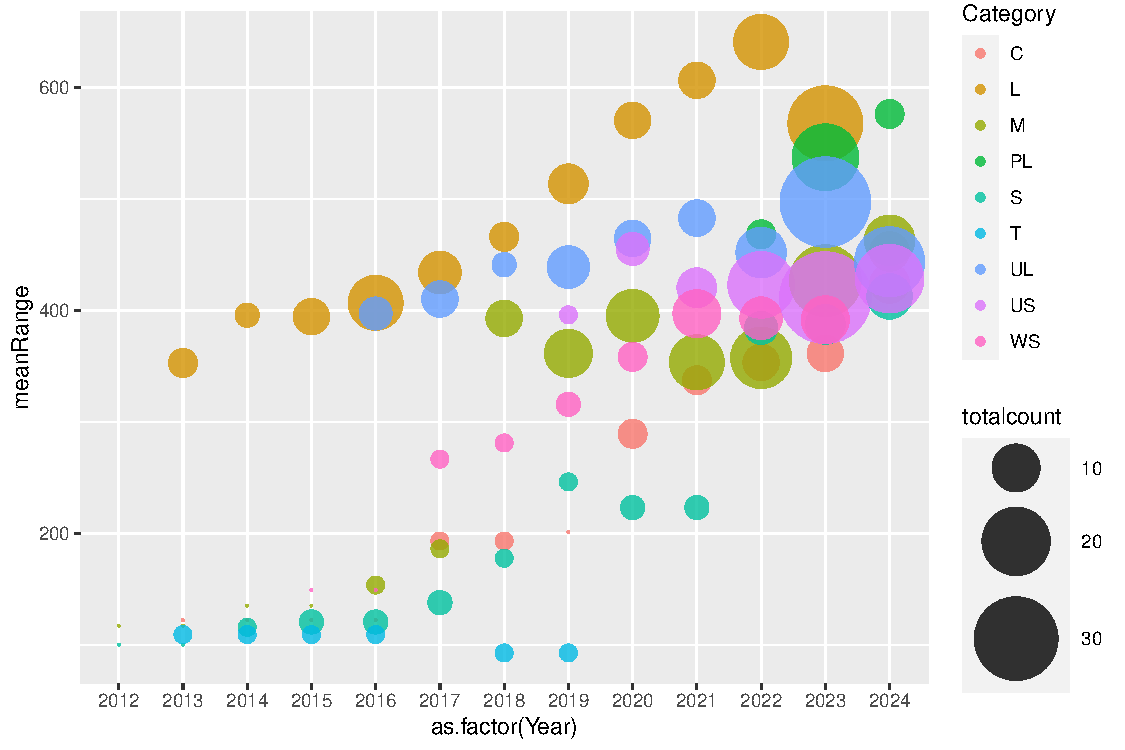
\includegraphics[height=1.75in]{fuel.pointsSize.pdf}
\end{column}
\begin{column}{.35\textwidth}
\footnotesize
\begin{itemize}
   \item Shows 4 variables
   \item Custom scale for point size
\end{itemize}
\end{column}
\end{columns}
\end{frame}

\begin{frame}[fragile]{Lines and Points Plot}
\begin{Rcode}
data |> 
  filter(Category %in% c('C','L','M','S','US','UL')) |>
  group_by(Year, Category) |>
  summarize(meanRange = mean(Range)) |>
  ungroup() |>
ggplot(aes(x=Year, y=meanRange, 
      color=Category, shape=Category, linetype=Category)) +
  geom_line(size=1) + 
  geom_point(size=4)  
\end{Rcode}
\begin{columns}
\begin{column}{.55\textwidth}
  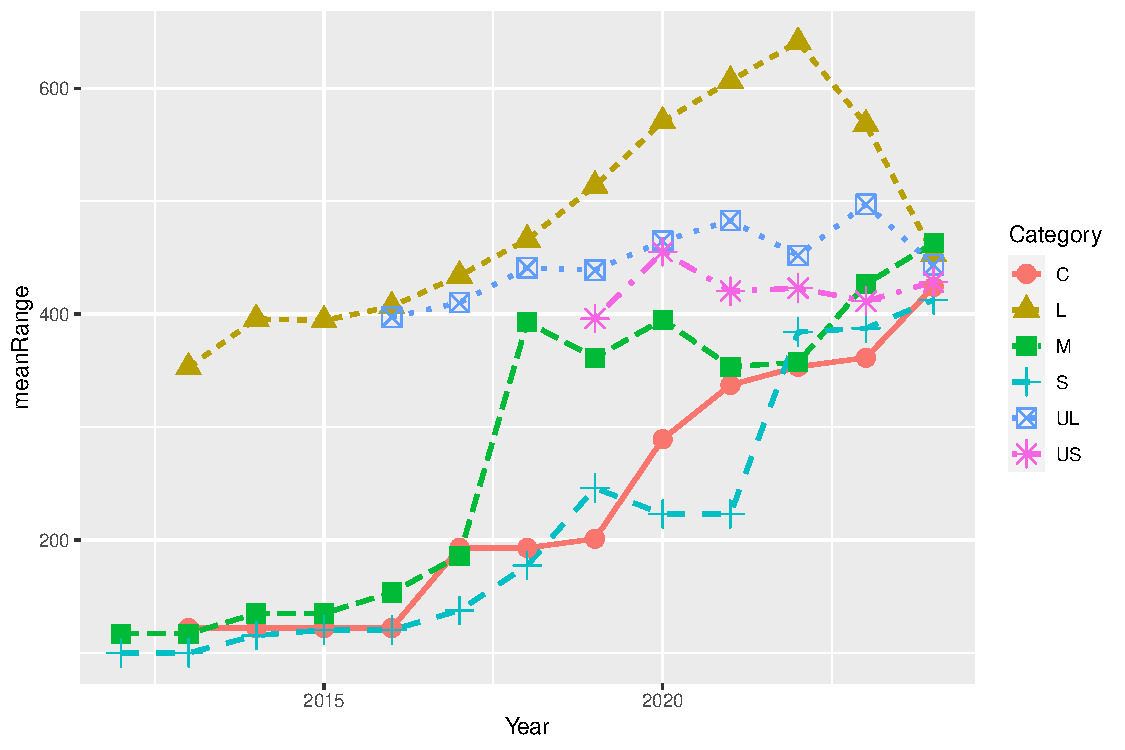
\includegraphics[height=1.5in]{fuel.linesPoints.pdf}
\end{column}
\begin{column}{.4\textwidth}
\footnotesize
\begin{itemize}
   \item 2 Geoms, line and point
   \item Category mapped to 3 plot elements
\end{itemize}
\end{column}
\end{columns}
\end{frame}

\begin{frame}[fragile]{Pie Chart}
\begin{columns}
\begin{column}{.55\textwidth}
\begin{Rcode}
data |>
  filter(Year==2023) |>
  group_by(Make) |>
  summarize(totalcount = n()) |>
  filter(totalcount >= 5) |>
  ungroup() |>
ggplot(aes(x='', y=totalcount, 
           fill=Make)) +
  geom_bar(stat='identity', 
           color='black', 
           size=0.25, width=1) + 
  coord_polar('y', 
              direction=-1, 
              start=0) +
  geom_text(aes(
    label=ifelse(totalcount >= 5,
                 totalcount,'')), 
    position = position_stack(
                 vjust=0.5)) +
  theme_void()
\end{Rcode}
\end{column}
\begin{column}{.55\textwidth}
  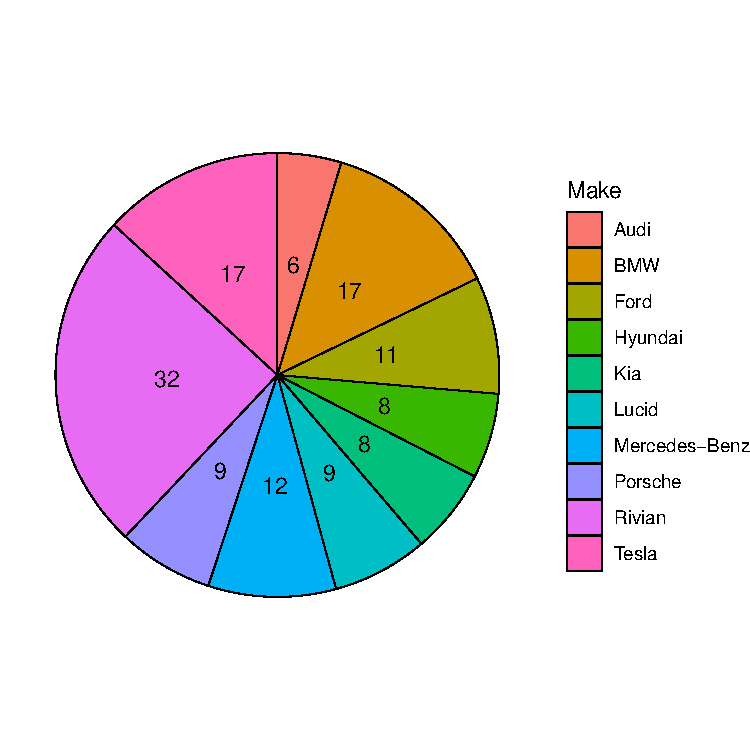
\includegraphics[width=\textwidth]{fuel.pie.pdf}
\end{column}
\end{columns}
\end{frame}


\begin{frame}{Pie Charts (XKCD)}
  \includegraphics[width=\textwidth]{xkcd_pie_charts.png}
\end{frame}

%\begin{frame}[fragile]{Donut Chart}
%\footnotesize
%\begin{minted}{R}
%holesize <- 2

%....

 %ggplot(aes(x=holesize, y=totalcount, fill=Make)) +
   %geom_col() + 
   %xlim(c(0.2, holesize+0.5)) +
     
%...

%\end{minted}
%\end{frame}

%\begin{frame}{Donut Chart}
%\centering
  %\includegraphics[width=.8\textwidth]{fuel.donut.pdf}
%\end{frame}

\begin{frame}[fragile]{Radar Plot}
Prepare data:
\begin{Rcode}
radardata <- data |>
  filter(Year == 2023) |> group_by(Make) |>
  summarize(meanCity = 1/mean(City), 
            meanHwy = 1/mean(Hwy), 
            meanRange = mean(Range)/100, 
            nModels = n()) |>
  filter(nModels >= 5) |> ungroup() |>
  select(-nModels) |>
  mutate(across(-Make, rescale))
\end{Rcode}

\footnotesize
\begin{itemize}
   \item The line \texttt{mutate(across(-Make, rescale))} rescales all columns except \texttt{Make} so values are between $[0,1]$
\end{itemize}

\begin{textcode}
# A tibble: 10 x 4
   Make          meanCity meanHwy meanRange
   <chr>            <dbl>   <dbl>     <dbl>
 1 Audi            0.122    0.270    0.0357
 2 BMW             0.202    0.360    0.219 
 3 Ford            0.287    0.182    0.220 
 4 Hyundai         1        0.630    0.260 
\end{textcode}
\end{frame}

\begin{frame}[fragile]{Radar Plot}
\begin{columns}
\begin{column}{.45\textwidth}
\begin{Rcode}
radardata |>  
  ggradar(
    axis.labels=c(
       'City', 
       'Highway', 
       'Range'), 
    values.radar='', 
    group.line.width=0.75, 
    group.point.size=3) +
  scale_color_ucscgb()
\end{Rcode}
\end{column}
\begin{column}{.65\textwidth}
  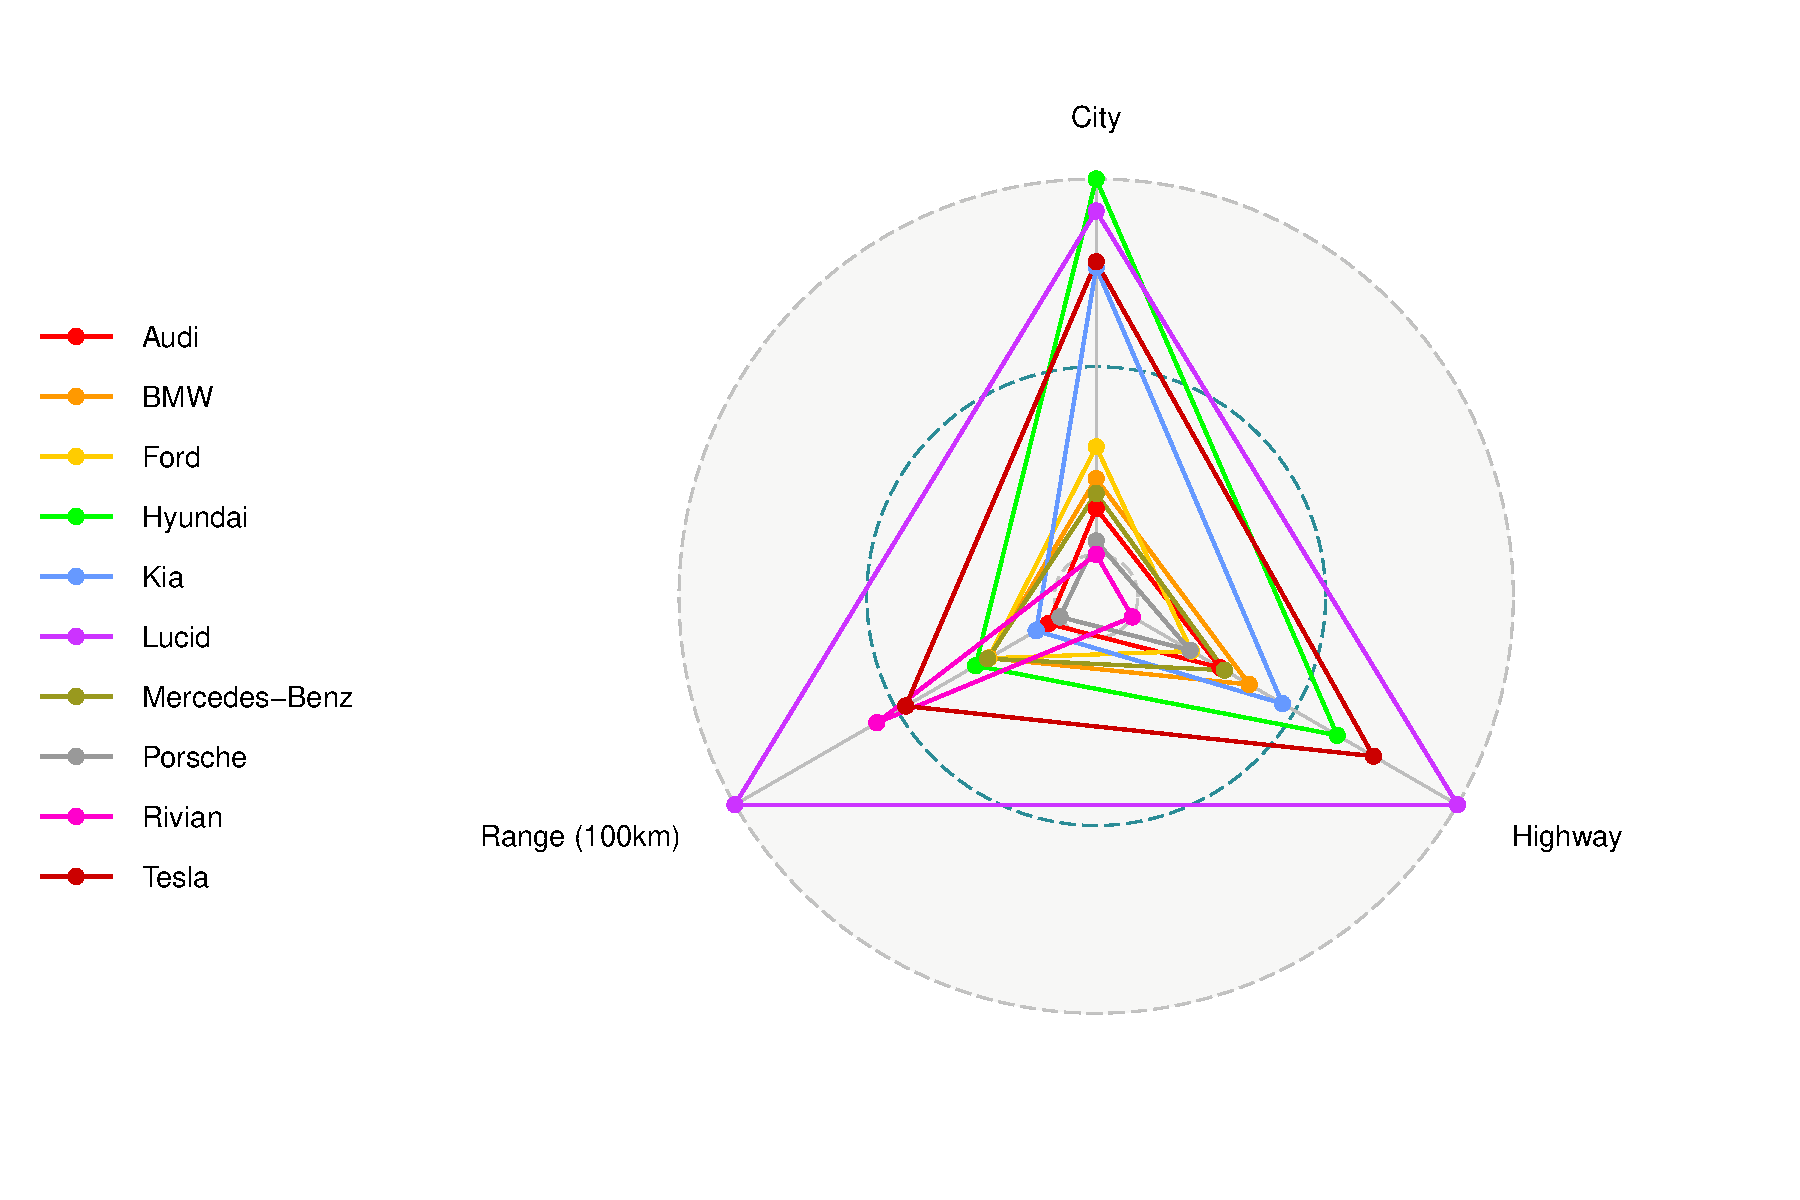
\includegraphics[width=.9\textwidth]{fuel.radar.pdf}
\end{column}
\end{columns}
\footnotesize
\begin{itemize}
   \item Shows a comparison of different objects on a number of dimensions/aspects. 
   \item Changed the colour palette to UCS CGB colours. 
\end{itemize}
\end{frame}



\begin{frame}[fragile]{Lines with Multiple Axes}
\footnotesize
\begin{Rcode}
data |>
   group_by(Year) |>
   summarize(meanCity = mean(City), 
             meanHwy = mean(Hwy), 
             meanRange = mean(Range)/100) |>
   ungroup() |>
ggplot(aes(x=Year)) +
  geom_line(aes(y=meanCity, color='Mean City')) + 
  geom_line(aes(y=meanHwy, color='Mean Hwy')) +
  geom_line(aes(y=meanRange, color='Mean Range')) +
  scale_color_manual(name='Data Series', 
     values=c('Mean City' = 'red', 
              'Mean Hwy' = 'blue', 
              'Mean Range' = 'green')) +
  scale_y_continuous(labels=scales::comma, 
      name="Fuel Consumption\n(l/100km equiv)", 
      sec.axis=sec_axis(~ .*100, 
                        labels=scales::comma, 
                        name="Mean Range (km)")) + 
  scale_x_continuous(breaks=seq(from=2012,to=2024,by=1))
\end{Rcode}
\end{frame}

\begin{frame}{Lines with Multiple Axes}
\begin{columns}
\begin{column}{.75\textwidth}
  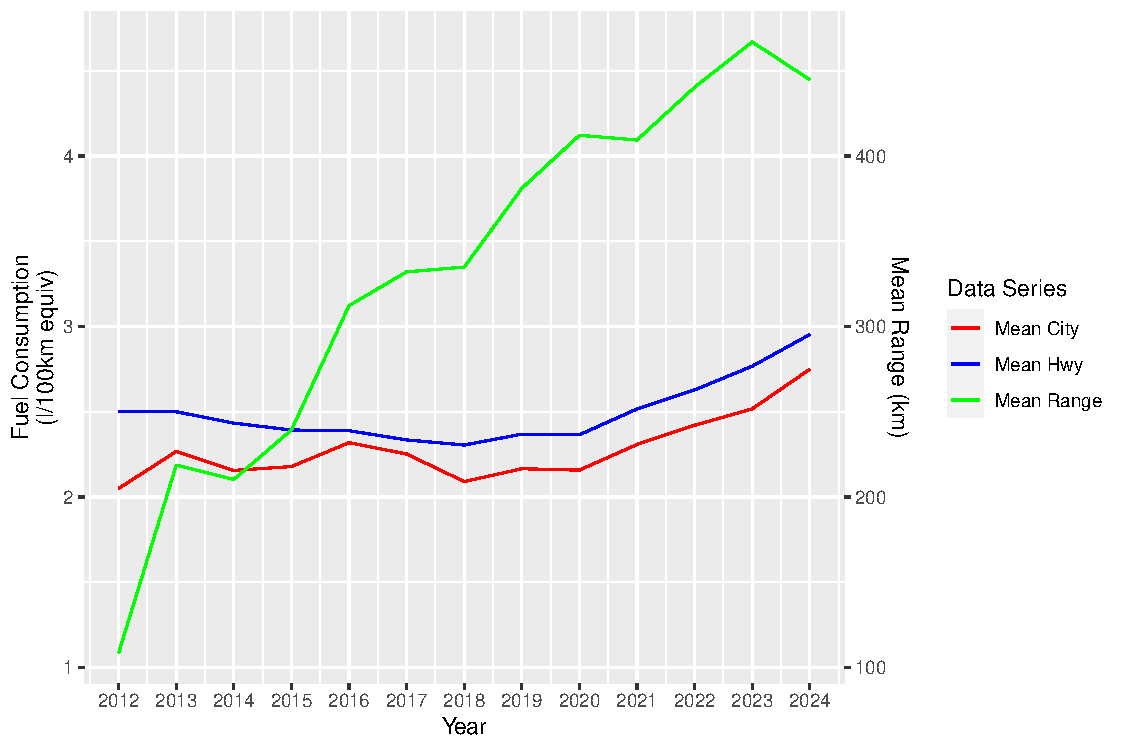
\includegraphics[width=\textwidth]{fuel.linesTwoScales.pdf}
\end{column}
\begin{column}{.35\textwidth}
\footnotesize
\begin{itemize}
   \item Three geoms
   \item Manual colour scale
   \item Y axis scale with primary label
   \item Secondary axis with \texttt{sec.axis} option, scale factor to primary axis, and secondary label
\end{itemize}
\end{column}
\end{columns}
\end{frame}

\begin{frame}[fragile]{Local Regression Smoothing Plot}
\footnotesize
\begin{Rcode}
data |>
  ggplot(aes(City, Hwy)) +
    geom_point() +
    geom_smooth()
\end{Rcode}
\begin{columns}
\begin{column}{.75\textwidth}
  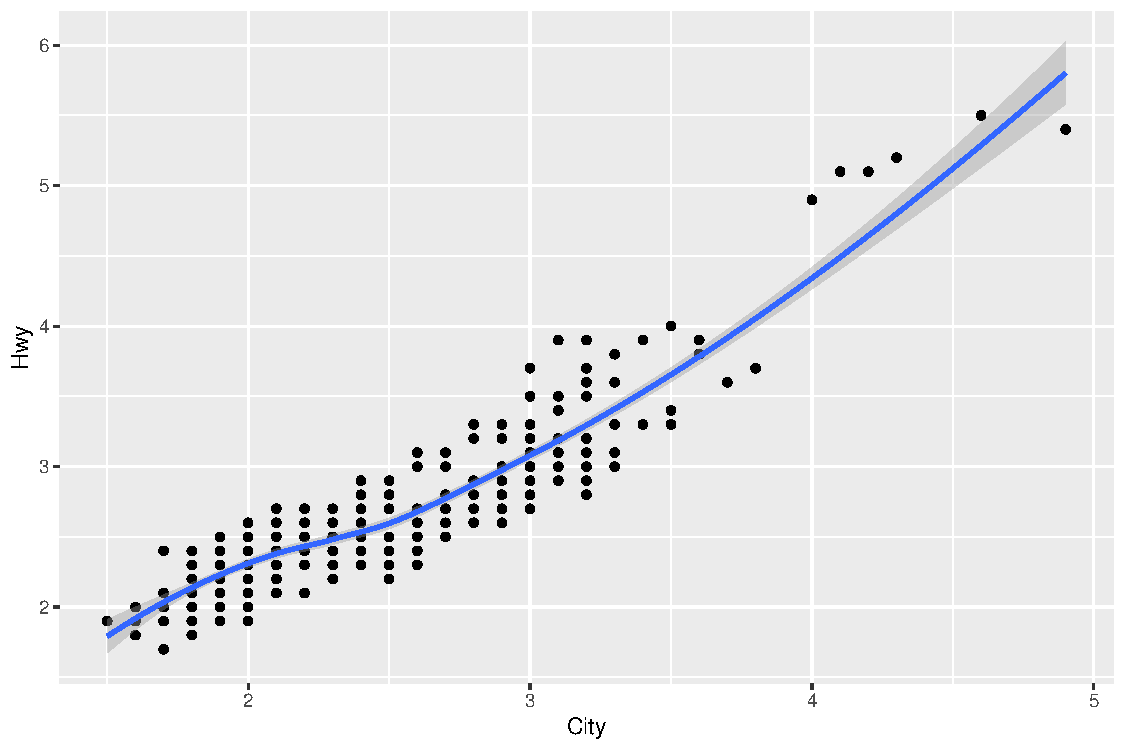
\includegraphics[width=\textwidth]{fuel.linesSmooth.pdf}
\end{column}
\begin{column}{.35\textwidth}
  \begin{itemize}
     \item Two geoms
     \item Local regression line
     \item Uncertainty interval around regression line
   \end{itemize}
\end{column}
\end{columns}
\end{frame}

%\begin{frame}[fragile]{Local Regression Smoothing Plot (with error bars)}
%\footnotesize
%\begin{Rcode}
%data %>% 
  %ggplot(aes(Year, Range)) +
    %geom_point() +
    %geom_smooth() +
    %stat_summary(
        %fun.data=mean_sdl, 
        %fun.args=list(mult=1), 
        %color='red', 
        %geom="errorbar") +
    %scale_y_continuous(labels=scales::comma) + 
    %labs(x = 'Year', color='', y = 'Mean Range (km)', 
    %title='Canadian Fuel Consumption Data', 
    %subtitle='2012 to 2024')
%\end{Rcode}
%\end{frame}

%\begin{frame}{Local Regression Smoothing Plot (with error bars)}
  %\includegraphics[width=\textwidth]{fuel.linesSmoothErrorBar.pdf}
%\end{frame}

%\begin{frame}[fragile]{Local Regression Smoothing Plot (with cross bars)}
%\footnotesize
%\begin{Rcode}
%data %>% 
  %ggplot(aes(Year, Range)) +
    %geom_point() +
    %geom_smooth() +
    %stat_summary(
        %fun.data=mean_sdl, 
        %fun.args=list(mult=1), 
        %color='red', 
        %geom="crossbar",
        %width=0.4) +
    %scale_y_continuous(labels=scales::comma) + 
    %labs(x = 'Year', color='', y = 'Mean Range (km)', 
    %title='Canadian Fuel Consumption Data', 
    %subtitle='2012 to 2024')
%\end{Rcode}
%\end{frame}

%\begin{frame}{Local Regression Smoothing Plot (with cross bars)}
  %\includegraphics[width=\textwidth]{fuel.linesSmoothCrossBar.pdf}
%\end{frame}

\begin{frame}[fragile]{2D Density Plot}
\begin{Rcode}
data |>
  ggplot(aes(x=Hwy, y=City)) + 
    geom_density_2d_filled() + 
    geom_density_2d() +
    geom_point(position='jitter')
\end{Rcode}
\begin{columns}
\begin{column}{.70\textwidth}
  \includegraphics[width=\textwidth]{fuel.density2d.pdf}
\end{column}
\begin{column}{.35\textwidth}
\begin{itemize}
  \item Shows (co-)distribution of observations
  \item Generalization of (1D) density plot
  \item Three geoms
  \item One for outline, one for fill, one for points
\end{itemize}
\end{column}
\end{columns}
\end{frame}

\begin{frame}[fragile]{2D Bin Plot}
\begin{Rcode}
data %>% 
  ggplot(aes(x=Hwy, y=City)) + 
    geom_bin2d(alpha=0.5, bins=10) +
    geom_point(color="black", size=1, position='jitter')
\end{Rcode}
\begin{columns}
\begin{column}{.70\textwidth}
  \includegraphics[width=\textwidth]{fuel.bin2d.pdf}
\end{column}
\begin{column}{.35\textwidth}
\begin{itemize}
  \item Shows (co-)distribution of observations
  \item Generalization of (1D) histogram plot
\end{itemize}
\end{column}
\end{columns}
\end{frame}

%\begin{frame}[fragile]{2D Bin Plot}
%\footnotesize
%\begin{Rcode}
%data %>% 
  %ggplot(aes(x=Hwy, y=City)) + 
    %geom_point(color="black", size=1, 
               %position='jitter') +
    %geom_bin2d(alpha=0.5, bins=5) + 
    %scale_x_continuous(labels=scales::comma) +
    %labs(x = 'Highway Consumption\n(l/100km equiv)', 
         %y = 'City Consumption\n(l/100km equiv)', 
         %fill='Count', 
         %title='Density Plot-Fuel Consumption Ratings', 
         %subtitle='Years 2012 to 2024') 
%\end{Rcode}
%\end{frame}

%\begin{frame}{2D Bin Plot}
  %\includegraphics[width=\textwidth]{fuel.bin2d.pdf}
%\end{frame}

%\begin{frame}[fragile]{2D Hex Plot}
%\footnotesize
%\begin{Rcode}
%data %>% 
  %ggplot(aes(x=Hwy, y=City)) + 
    %geom_point(color="black", size=1, 
               %position='jitter') +
    %geom_hex(alpha=0.5, bins=5) + 
    %scale_fill_distiller(palette=4, direction=-1) +
    %scale_x_continuous(labels=scales::comma) +
    %labs(x = 'Highway Consumption\n(l/100km equiv)', 
         %y = 'City Consumption\n(l/100km equiv)', 
         %fill='Count', 
         %title='Density Plot-Fuel Consumption Ratings', 
         %subtitle='Years 2012 to 2024') 
%\end{Rcode}
%\end{frame}

%\begin{frame}{2D Hex Plot}
  %\includegraphics[width=\textwidth]{fuel.hex2d.pdf}
%\end{frame}

\begin{frame}[fragile]{3D Raster/Tile Plot}
\footnotesize
\begin{Rcode}
data |>
  ggplot(aes(x=Hwy, y=City, fill=Range)) + 
    geom_tile() 
\end{Rcode}
\begin{columns}
\begin{column}{.75\textwidth}
  \includegraphics[width=\textwidth]{fuel.raster.pdf}
\end{column}
\begin{column}{.25\textwidth}
\begin{itemize}
  \item Plot of three variables
\end{itemize}
\end{column}
\end{columns}
\end{frame}

\begin{frame}[fragile]{Complex Example -- 3D Raster Plot with Rug}
\begin{Rcode}
data |>
  ggplot(aes(x=Hwy, y=City, fill=Range)) + 
    geom_tile() + 
    geom_point(size=0.5, position='jitter') +
    geom_rug(position='jitter') + 
    scale_fill_distiller(palette=4, direction=-1)
\end{Rcode}
\begin{columns}
\begin{column}{.65\textwidth}
  \includegraphics[width=\textwidth]{fuel.raster.rug.pdf}
\end{column}
\begin{column}{.35\textwidth}
\begin{itemize}
  \item Geom for tiling
  \item Geom for points/observations
  \item Geom for ''rugs''
  \item Custom colour scale
\end{itemize}
\end{column}
\end{columns}
\end{frame}

\begin{frame}{Hands-On Exercises}
\footnotesize
Using the Pagila database data from \url{https://evermann.ca/busi4720/rentals.csv}, create
\begin{enumerate}
   \item A histogram and/or density chart of film length by film category
   \item A column chart of the mean rental payments for films by film category
   \item A scatter plot of total rental payments by year and week
   \begin{itemize}
	  \footnotesize
      \item Add a local regression line to this plot
   \end{itemize}
   \item A pie or donut chart of rental counts by film rating
\end{enumerate}
\textbf{Tips:}
\begin{itemize}
\item Use the \texttt{read\_csv()} function to read from a URL
\item The data is de-normalized, use the \texttt{unique()} function to get accurate film counts
\item Use the \texttt{year()} and \texttt{week()} functions from the \texttt{lubridate} package (another package of the Tidyverse set)
\end{itemize}
\end{frame}


\end{document}
